\documentclass[a4paper,11pt]{article}

\usepackage[affil-it]{authblk}
%\usepackage{amsfonts, amsmath, amssymb, bm}
%\usepackage{float}
\usepackage[margin=1.0in]{geometry}
\usepackage{graphicx}
%\usepackage{hyperref}
%\usepackage{subcaption}
%\usepackage{subfigure}
\usepackage{url}

%\graphicspath{{../pdf/}{../jpeg/}}
% \DeclareGraphicsExtensions{.pdf,.jpeg,.png}
\graphicspath{{figures/}}

%\newcommand{\bfnull}{\textbf{null}}

\begin{document}

\title{Towards the Planning of World Domination}
\author{Jason Gregory and Kamruzzaman Quddus \\ \{jgregory, kquddus\}@umd.edu}
\affil{University of Maryland, College Park, MD}
\date{\today}

\maketitle

%
\abstract{Abstract goes here.}

\section{Introduction}\label{sec:intro}
High-level overview of topic and introduction of problem statement: Warlight AI Challenge 2.

\subsection{Problem Statement}\label{sec:problem}
Seeking to develop a robust planner for the Warlight AI Challenge 2 \cite{warlight}.
Describe rules of Warlight game (our bot vs one opponent, random map, fog of war, standard scoring and troop allocation, no cards).

\subsection{Previous Work}\label{sec:previous}
Reference other bots in challenge, publications on risk strategies, etc.

\subsection{Importance and Relevancy}\label{sec:importance}
What remains - Own implementation of planning algorithm using topics covered in this class.
Why interesting - Demonstrate topics from class in real-world example.
What is significance - Application of theoretical concepts to interesting game (and world domination)

%
\section{Technical Approach}\label{sec:approach}
High-level description of approach.

\subsection{Hypothesis}\label{sec:hypothesis}
We think a Refinement Acting Engine (RAE), SeRPE, or HTN (not sure which) will fit well into this structure and application.

\subsection{Process}\label{sec:process}
Describe how we plan to apply the RAE/SeRPE/HTN solution to this problem. 
High-level description of implementation. 
Evaluation will be via implementation and simulation (game engine).
Metric is (1) score compared to other bots and/or (2) score of each of our own implementations.
Maybe implement a few planners and compare performance against one another.

%
\section{Project Management}\label{sec:management}
The main tasks of this project include implementing the UCT algorithm, conducting simulations, and evaluating the generated data so that we can publish our results in a report and a presentation. 

\subsection{Tasks}\label{sec:tasks}
There are seven main tasks required to successfully develop a planner that is capable of winning a game in the Warlight AI Challenge 2.  The first, which we have already completed, is a literature review of the UCT algorithm, its variants, and its application to the planning of games involving artificial intelligence. The next task is formulating the problem in a manner that is compatible with our proposed approach. With a concrete understanding for a possible solution, the next task is to implement the basic UCT algorithm.  The next two tasks consist of testing, modifying and improving our implementation to enhance the performance of our solution.  A simulation and evaluation of our algorithm is required to determine how well it performs compared to other strategies. Finally, we will present our results in a report and a presentation.  These tasks, with their respective tentative deadlines and durations are summarized in Table~\ref{tab:deadlines} and Figure 1. %~\ref{fig:gantt}.

%
\begin{table}[tbp]
  \centering
  \begin{tabular}{|c|c|}
    \hline
    \emph{Task} & \emph{Deadline} \\ 
    \hline
    Literature Review & March 9, 2015 \\ \hline
    Problem Formulation & March 16, 2015 \\ \hline
    UCT Implementation & April 6, 2015 \\ \hline
    Testing & April 13, 2015 \\ \hline
    UCT Modification and Improvement & April 13, 2015 \\ \hline
    Simulation and Evaluation & April 27, 2015 \\ \hline
    Write Report and Presentation & May 2, 2015 \\ \hline
  \end{tabular}
  \caption{Table of deadlines.}
  \label{tab:deadlines}
\end{table}

%
\begin{figure}[tbp]
  \centering
  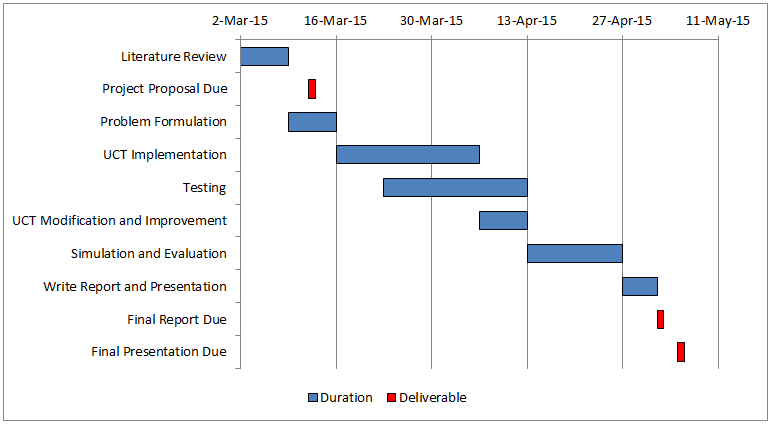
\includegraphics[width=0.95\columnwidth]{gantt_chart}
  \label{fig:gantt}
  \caption{Gantt chart}
\end{figure}

\subsection{Assignments}\label{sec:assignments}
Divide and conquer tasks, WAR code, etc.

\subsection{Schedule}\label{sec:schedule}
Gantt chart with milestones and dates.

%
\section{Conclusions}\label{sec:conclusions}
Summary of problem and intended approach.

% References 
\bibliographystyle{plain}
\bibliography{references}

% End document
\end{document}

